%%%%%%%%%%%%%%%%%%%%%%%%%%%%%%%%%%%%%%%%%%%%%%
% Header
\documentclass[12pt]{article}
\usepackage[english]{babel}
\usepackage[utf8x]{inputenc}
\usepackage{hyperref}
\usepackage{graphicx}
\usepackage{fullpage}
\usepackage[lastexercise]{exercise}
\usepackage{enumitem}
\graphicspath{ {./img/} }

\setlength{\parindent}{0cm}

\renewcommand{\ExerciseHeader}{\large\textbf{\ExerciseName~\ExerciseHeaderNB} - \textbf{\ExerciseTitle}\medskip}

\renewcommand{\ExePartHeader}{\medskip\textbf{\ExePartName\ExePartHeaderNB\ExePartHeaderTitle\medskip}}

\begin{document}
%%%%%%%%%%%%%%%%%%%%%%%%%%%%%%%%%%%%%%%%%%%%%%
\title{Exercises -- Week 1: Introduction to Python}
\subsubsection*{EMAT10007 -- Introduction to Computer Programming}
\subsection*{\Large Exercises -- Week 1. Introduction to Python, Variables and Operators}

\section*{Introduction}

\subsection*{Getting Started}

\begin{itemize}

    
    \item{To open Anaconda on a Linux lab computer
    
    \begin{itemize}
        \item{Click on Activities in the top left corner of the screen.}
        \item{Open 'Terminal' from the menu tab.}
        \item{Type or copy and paste the following:  
        
        \vspace{0.5em}
		{\tt /opt/anaconda/2020.07/bin/anaconda-navigator}
	    \vspace{0.5em}
	    }
	    \item{Press enter}
    \end{itemize}
    }
    
    \item{{\bf [If completing these exercises off-campus/on your personal laptop}, first install Anaconda by following the instructions in the links on blackboard {\bf or} use remote desktop to access a lab computer, then choose Anaconda from the programs menu.]} 

    \item{Launch Spyder IDE from the Anaconda Navigator window by clicking on the Launch button next to the Spyder logo - we will use Spyder to write and run Python code.}
    \item{Complete the exercises using the Spyder IDE, save your work as a .py file.}
    \item{Try to complete all of the {\bf Essential} questions in the lab.}
    \item{Complete any unfinished {\bf Essential} questions for homework before the next class.}
    \item{The {\bf Advanced} questions are optional. You may attempt these if you have finished the Essential questions.}
\end{itemize}

\subsection*{Creating, saving and opening Python files in the Spyder IDE}
     
\begin{itemize}
    \item To create a new Python file click ``File'' and then ``New File''.
    \item Write some code.
    \item To save a Python file click ``File'' and then ``Save''.
    \item If this is the first time you are saving the file, you will be prompted to choose a file name and location. Name your file and save it somewhere appropriate with .py extension. 
    \item Next time you open Spyder, you can access the file by clicking on ``File'' then ``Open'', and then navigating to where your file is stored.
\end{itemize}
    

\subsection*{Rules for naming variables}
	\begin{itemize}
        \item Variables can be assigned values
        \item Variable names may contain letters or numbers
        \item Variable names must begin with a letter
        \item Variable names are case sensitive ({\tt time} is not the same as {\tt Time})
        \item The value of the variable can be re-assigned. If we have {\tt x = 1} in a program followed by {\tt x = 2}, the original value of {\tt x} will be overwritten with the new value, 2. 
        \item We can also assign multiple variables on the same line.
	
	    \vspace{0.5em}
		{\tt x, y  = 5, 10}
		\vspace{0.5em}
		
        \item Some {\tt keywords} are reserved by the Python language and cannot be used as variable names. For a full list of keywords reserved by Python, enter the following in Spyder and press Run:
		
		\vspace{0.5em}
		{\tt import keyword}
		
		{\tt print(keyword.kwlist)}
		\vspace{0.5em}
		
		\item{Use a consistent naming convention such as {\tt snake\_case} when naming variables.}
		
    \end{itemize}
    
\section*{Part 1 - Variables}

%\subsection*{Essential Questions}

\begin{Exercise}[title=Numbers and Arithmetic Operators (Essential)]  \label{Ex:Numbers}

\ExeText{Python can be used as a calculator. You can input operations, and store the results of operations as variables for use in additional calculations.}
	\Question{Create two variables, {\tt a} and {\tt b}, and assign a numerical value of your choice to each of these variables.}
	\Question{Calculate the sum of {\tt a} and {\tt b} and print the result in the Console window in Spyder.}
	\Question{Calculate the product of {\tt a} and {\tt b} and store the result as a new variable.}
	\Question{Overwrite the value of the variable you just created with the value $\frac{a+b}{3}$. \\Hint: Python follows the same ordering of mathematical operations as any other calculator.
	\Question{Find the remainder when {\tt a} is divided by {\tt b} and print the result.}.
    % \Question{Write a program that stores the radius of a sphere as a variable, then finds the volume of the sphere as a new variable.}\label{Q:Sphere}
    \Question{In a single line of code, create 3 variables for the length, width and height of a cuboid. Then, write a program to store the volume of the cuboid as a new variable.}\label{Q:Cuboid}
    \end{Exercise}

\begin{Exercise}[title=Strings (Essential)] \label{Ex:Strings}

Strings are text data. 

% \ExeText{Strings behave differently from numerical data. 

% We can return the Nth character(s) of a string with {\tt string[N]} e.g. 

%         \vspace{0.5em}
% 		{\tt x = `Hello'} 
		
% 		{\tt print(x[0]) }
		
% 		{\tt \bf  `H' }
		
% 		\vspace{0.5em}
% 		{\tt print(x[0:3]) }
		
		
% 		{\tt \bf `Hel' }
% 		\vspace{0.5em}}
		


    \Question{Create two variables {\tt c} and  {\tt d}. Assign the value {\tt `Hello'} to {\tt c} and  the value {\tt `World'} to {\tt d}. }
    \Question{ Use arithmetic operators and these variables to create a new string variable with the value: {\tt `Hello World'}}
	\Question{Print the third letter of {\tt c}.}
	\Question{Print the last three letters of {\tt d}}

\end{Exercise}

\begin{Exercise}[title=Modelling with Variables (Essential)]  \label{Ex:Modelling}

    \Question{Write a program that finds the volume of a sphere and the area of the cross section that passes through its centre, using its radius, and then displays these values.}\label{Q:Sphere}

\end{Exercise}


%\subsection*{Advanced Questions}

\begin{Exercise}[title=More Variables (Advanced)] 

    \Question{Practise expressing some simple mathematical expressions of your own using arithmetic operations.}
    \Question{What happens if you use arithmetic operators on Boolean ({\tt True} or {\tt False}) values?}


\end{Exercise}	

%\section*{Part 2 - Operators}

%\subsection*{Essential Questions}

\begin{Exercise}[title=Comparison Operators (Essential)]

\ExeText{Comparison Operators output a {\tt True} or {\tt False} (Boolean) value.\\ Use variables {\tt a} and {\tt b} (from Exercise \ref{Ex:Numbers}), and {\tt c} and {\tt d} (defined in  Exercise \ref{Ex:Strings}) for these exercises.}

	\Question{Write a line of code that prints {\tt True} in the Console window in Spyder if variable {\tt a} is greater than {\tt b}}.
	\Question{Write a line of code that prints {\tt True} if the {\tt type} of {\tt a} is the same as {\tt b}. Can you change the value of {\tt a} and/or {\tt b} to output a different result?}
	\Question{Write a line of code that prints {\tt True} if the first letter of {\tt c} is the same as the first letter of {\tt d}. Change the value of {\tt c} and {\tt d} to check your code works as expected}.
% 	\Question{Write a program that compares the volume of a sphere found in Exercise \ref{Ex:Numbers}.\ref{Q:Sphere} the volume of the cuboid found in Exercise \ref{Ex:Numbers}.\ref{Q:Cuboid} and outputs a message telling the user which is larger e.g.}
	
% 	        \vspace{0.5em}
%     		{\tt `The volume of the sphere is greater: True'}
    		
%     		{\tt `The volume of the cuboid is greater: False'}
	
	
	
\end{Exercise}
	




\begin{Exercise}[title=Logical Operators (Essential)]

\ExeText{Logical Operators output a {\tt True} or {\tt False} (Boolean) value.\\ Use variables {\tt a}, {\tt b} Exercise \ref{Ex:Numbers} for these exercises.}

\ExeText{}
	
	\Question{Write a line of code that prints {\tt True} in the Console window in Spyder if both variables {\tt a} {\bf and} {\tt b} are even.}
	\Question{Write a line of code that prints {\tt True} if either variable {\tt a} {\bf or} {\tt b} is even.} 
	\Question{Create three variables in a single line of code. Each variable should be the name of a student and the value of the variable should be their score in an imaginary assignment e.g {\tt Valentina = 75}. The pass mark for the assignment is 40. Write a program that outputs {\tt True} if any of the three students passed the assignment.}
\end{Exercise}

\begin{Exercise}[title=Modelling with Operators (Essential)]  \label{Ex:Modelling}

	\Question{Write a program that compares the volume of a sphere and the volume of a cuboid and outputs a message telling the user which is larger e.g.}

        \vspace{0.5em}
		{\tt `The volume of the sphere is greater: True'}
		
		{\tt `The volume of the cuboid is greater: False'}
		
	\Question{Write a program that sorts animals into three categories: herbivores, carnivores and omnivores based on two facts about the animal: (1) whether or not it eats meat and (2) whether or not it eats plants.}

\end{Exercise}

%\subsection*{Advanced Questions}

\begin{Exercise}[title=More Operators (Advanced)] 


    % \item Write a program that sorts animals into three categories: herbivores, carnivores and omnivores based on two variables that indicate if the animal eats plants and/or eats meat.
    
    \Question{Create a variable with a numerical value. Write a program that prints {\tt True} if the number is a square number or perfect square (i.e. the product of some integer with itself).}
    
    % \begin{figure}[h]
    % \centering
    % 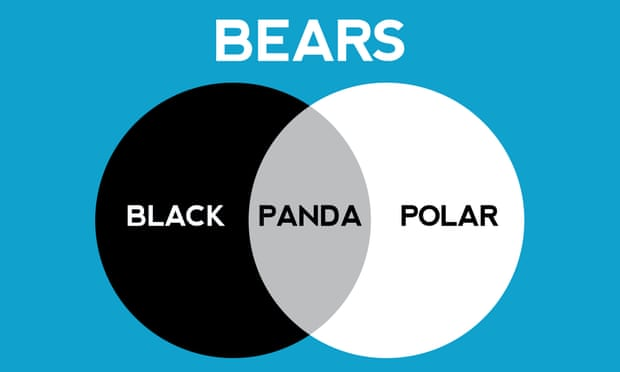
\includegraphics[scale = 0.5]{bears_} 
    % \end{figure}
    
    \Question{Write a program, like the example shown in today's class, based on your own typical day, that tells you what action to do based on the time of day.}  
    
\end{Exercise}





\subsection*{Checklist}
\begin{itemize}
	\item Check that you understand the basics: variables, different types of variables (numbers (integers, floats), Booleans, strings), the different types of operators, and how these work with both numbers and strings.
	\item Finish any incomplete Essential exercises for homework. 
	\item Attend the drop-in session for one-to-one support from a Teaching Assistant if there was anything you didn't understand.
\end{itemize}


\end{document}